\documentclass[10pt, oneside,a4paper]{article}
\usepackage[text={170mm, 230mm}, vmarginratio=1:1]{geometry}
\usepackage[usenames,dvipsnames]{color}
\usepackage{colortbl}
\definecolor{mygray}{gray}{.9}
\usepackage[slantfont,boldfont]{xeCJK}
\setCJKmainfont{SimSun}
\usepackage{array}
\usepackage{tabularx}
\usepackage[colorlinks, linkcolor=black, anchorcolor=blue, citecolor=green]{hyperref}
\usepackage{upgreek}
\usepackage{xcolor, color}
\usepackage[framemethod=tikz]{mdframed}
\usepackage{graphicx, psfrag}
\usepackage{fancyhdr}
\pagestyle{fancy}
\usepackage{indentfirst}
\usepackage{threeparttable}
\usepackage{float}
\linespread{1.5}
\setlength{\parindent}{2em}
\renewcommand{\headrulewidth}{0pt}
\setlength{\headheight}{20 pt}
\hfuzz=\maxdimen
\tolerance=10000
\hbadness=10000
\lhead{}
\chead{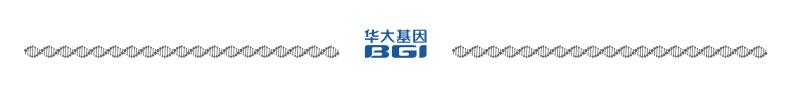
\includegraphics[width=180 mm, keepaspectratio]{./source/bgi_title.jpg}}
\rhead{}
\lfoot{深圳华大基因}
\cfoot{\thepage}
\rfoot{2017 BGI All Rights Reserved.}
\begin{document}
\vspace{50 mm}
\title{
\includegraphics[width=80 mm, keepaspectratio]{./source/BGI-LOGO2.png}}
\maketitle
\vspace{30 mm}
\begin{center}
\huge{\textbf {生物信息分析报告}}\par
\vspace{50 mm}
\textbf{\large{华大基因生物技术有限公司}}\par
\end{center}
\newpage
\renewcommand{\contentsname}{目录}
\tableofcontents
\newpage
\section{项目概况}
\vspace{25 mm}
\textbf{\textit{\large{项目名称: }}\large{rice mRNAseq}}\par
\vspace{5 mm}
\textbf{\textit{\large{客户名称: }}\large{yueyao}}\par
\vspace{5 mm}
\textbf{\textit{\large{客户单位: }}\large{华大基因}}\par
\vspace{5 mm}
\textbf{\textit{\large{项目编号: }}\large{000001}}\par
\vspace{5 mm}
\textbf{\textit{\large{物\hspace{2 em}种: }}\large{rice}}\par
\vspace{5 mm}
\textbf{\textit{\large{样本数量: }}\large{CK-1}}\par
\newpage
\section{建库测序流程}
从RNA样品到最终测序数据的分析,样品检测、建库、测序每一个环节都会对数据质量和数量产生影响,而数据质量又会直接影响后续信息分析的结果。
为了从源头上保证测序数据的准确性、可靠性,华大对样品检测、建库、测序每一个生产步骤都严格把控,从根本上确保了高质量数据的产出。流程图如下:
\begin{center}
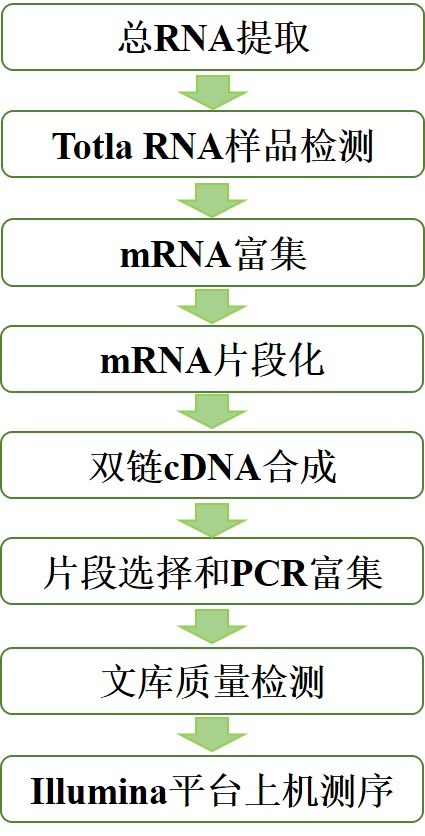
\includegraphics[width=45 mm, keepaspectratio]{./source/library_cst.jpg}
\end{center}
\subsection{Total RNA样品检测}
对RNA样品的检测主要包括4种方法:
\begin{itemize}
\item 琼脂糖凝胶电泳分析RNA降解程度以及是否有污染
\item Nanodrop检测RNA的纯度(OD260/280比值)
\item Qubit对RNA浓度进行精确定量
\item Agilent2100精确检测RNA的完整性
\end{itemize}
\subsection{文库构建}
样品检测合格后,用带有Oligo(dT)的磁珠富集真核生物mRNA(若为原核生物,则通过试剂盒去除rRNA来富集mRNA)。随后加入fragmentation buffer将mRNA打断成短片段,以mRNA为模板,用六碱基随机引物(random hexamers)合成一链cDNA,然后加入缓冲液、dNTPs和DNA polymerase I合成二链 cDNA,随后利用AMPure XP beads纯化双链cDNA。纯化的双链cDNA再进行末端修复、加A尾并连接测序接头,然后用AMPure XP beads进行片段大小选择,最后进行PCR富集得到最终的cDNA文库。构建原理图如下:
\begin{center}
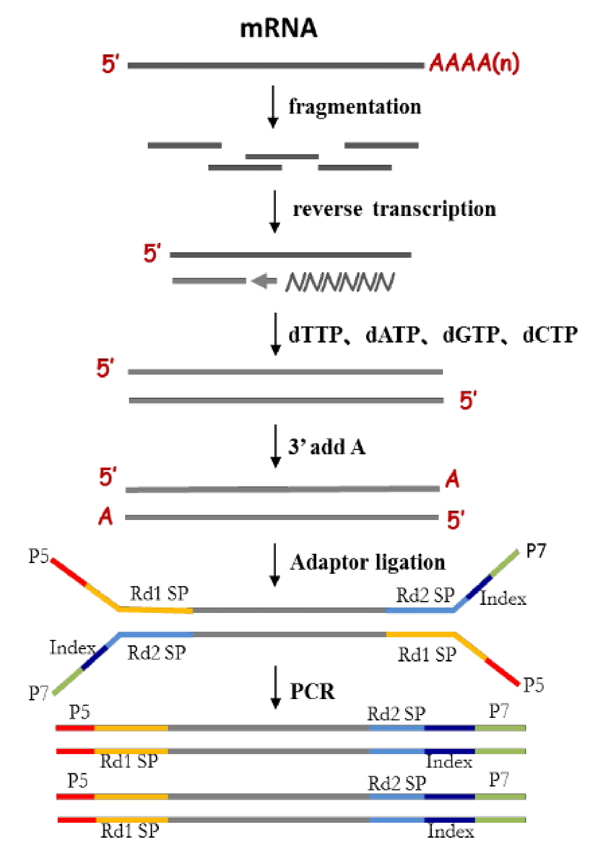
\includegraphics[width=60 mm, keepaspectratio]{./source/library_process.jpg}
\end{center}
\section{生物信息分析流程}
首先对原始下机数据(raw data)进行过滤,将过滤后得到的高质量序列(clean data)比对到该物种的参考基因组上。 
根据比对结果,计算每个基因的表达量。 在此基础上,进一步对样品进行表达差异分析、富集分析和聚类分析。
\begin{center}
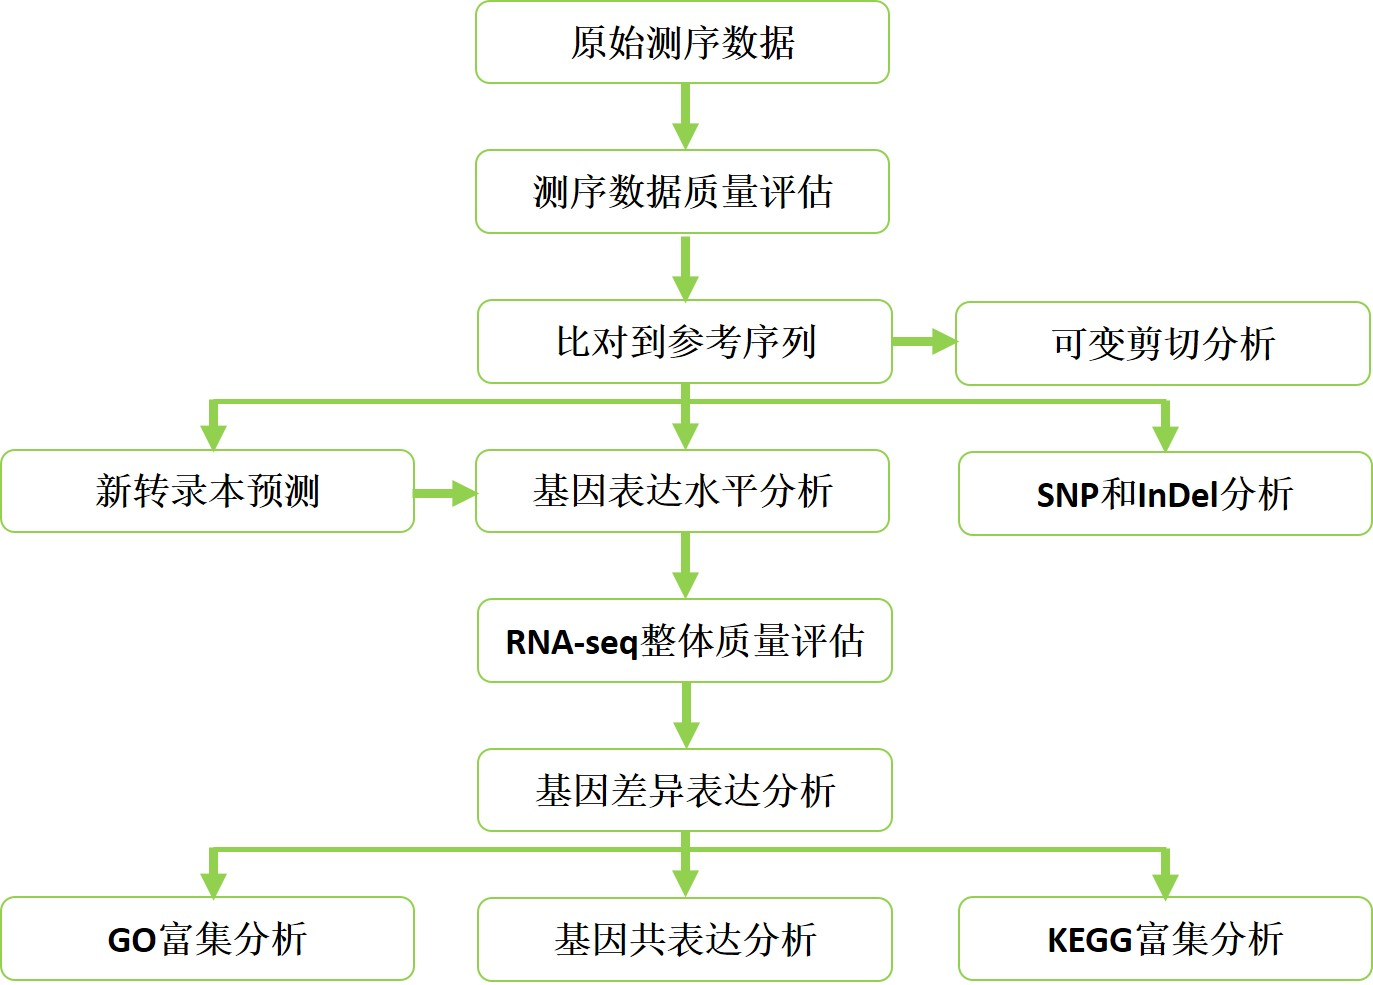
\includegraphics[width=100 mm, keepaspectratio]{./source/als_proc.jpg}
\end{center}
\newpage
\section{结果展示及说明}
\subsection{原始序列数据}
高通量测序 (如Illumina HiSeq$^{TM}$ 2500/Miseq$^{TM}$ )得到的原始图像数据文件经CASAVA碱基识别(Base Calling)分析
转化为原始测序序列(Sequenced Reads),我们称之为Raw Data或Raw Reads,
结果以FASTQ(简称为fq)文件格式存储,其中包含测序序列(reads)的序列信息以及其对应的测序质量信息。\par
FASTQ格式文件中每个read由四行描述,如下:\par
@HWI-ST1276:71:C1162ACXX:1:1101:1208:2458 1:N:0:CGATGT\par
NAAGAACACGTTCGGTCACCTCAGCACACTTGTGAATGTCATGGGATCCAT\par
+\par
\#55???BBBBB?BA@DEEFFCFFHHFFCFFHHHHHHHFAE0ECFFD/AEHH\par
其中第一行以'@'开头,随后为Illumina测序标识符(Sequence Identifiers)和描述文字(选择性部分);\par
第二行是碱基序列;\par
第三行以'+'开头,随后为Illumina测序标识符(选择性部分);\par
第四行是对应碱基的测序质量,该行中每个字符对应的ASCII值减去33,即为对应第二行碱基的测序质量值。\par
测序样本序列见文件夹$\href{run:./BGI\_result/1.CleanData}{/BGI\_result/1.CleanData}$文件夹\par
\subsection{测序数据质量评估}
\subsubsection{测序错误率分布检查}
每个碱基测序错误率是通过测序 Phred数值 (Phred score, Q phred)通过公式(公式 1 : Qphred = -10$\log_{10}e$)转化得到,
而Phred数值是在碱基识别(Base Calling)过程中通过一种概率模型计算得到,这种模型可以准确地预测碱基判别的错误率。
Phred分值,不正确的碱基识别率,碱基正确识别率以及Q-score的对应关系如下表所显示:\par
illumina Casava 1.8 版本碱基识别与Phred分值之间的简明对应关系\par
\vspace{3 mm}
\begin{center}
\begin{tabularx}{110mm}{cccc}
\hline
\textbf{Phred分值} & \textbf{不正确的碱基识别} & \textbf{碱基正确识别率} & \textbf{Q-Score} \\
\hline
10 & 1/10 & 90\% & Q10 \\
20 & 1/100 & 99\% & Q20 \\
30 & 1/1000 & 99.9\% & Q30 \\
40 & 1/10000 & 99.99\% & Q40 \\
\hline
\end{tabularx}
\end{center}
\vspace{5 mm}
\par
测序错误率与碱基质量有关,受测序仪本身、测序试剂、样品等多个因素共同影响。对于RNA-seq技术,测序错误率分布具有两个特点:\par
(1)测序错误率会随着测序序列(Sequenced Reads)长度的增加而升高,这是由于测序过程中化学试剂的消耗导致的,并且为
illumina高通量测序平台都具有的特征。\par
(2)前6个碱基的位置也会发生较高的测序错误率,而这个长度也正好等于在RNA-seq建库过程中反转录所需要的随机引物的长度。
所以前 6个碱基测序错误率较高的原因为随机引物和RNA模版的不完全结合。\par
\subsubsection{测序数据过滤}
测序得到的原始测序序列,里面含有带接头的、低质量的reads,为了保证信息分析质量,必须对raw reads进行过滤,得到clean reads,
后续分析都基于clean reads。\par
数据处理的步骤如下:\par
(1) 去除带接头(adapter)的reads;\par
(2) 去除N(N表示无法确定碱基信息)的比例大于10\%的reads;\par
(3) 去除低质量reads(质量值sQ <= 5的碱基数占整个read长度的50%以上的reads)\par
过滤后reads的质量指标见表\ref{ReadsStatistic},碱基含量分布以及质量分布见图\ref{ReadsBase}和图\ref{ReadsHeatmap}\par
测序样本序列比对到基因组结果见文件夹$\href{run:./BGI\_result/1.CleanData}{./BGI\_result/1.CleanData}$文件夹\par
\vspace{5 mm}
\begin{table}[h]
\centering
\resizebox{\textwidth}{!}{
\begin{threeparttable}
\centering\caption{过滤后的reads质量统计}\label{ReadsStatistic}
\renewcommand{\tablename}{表}
\begin{tabular}{*{7}c}
\hline
\rowcolor{blue!60}
\textbf{Sample} & \textbf{Total Raw Reads(Mb)} & \textbf{Total Clean Reads(Gb)} & \textbf{Total Clean Bases(Gb)} & \textbf{Clean Reads Q20(\%)} & \textbf{Clean Reads Q30(\%)} & \textbf{Clean Reads Ratio(\%)} \\
\hline
CK-1 & 61.94 & 61.94 & 9.29 & 96.98 & 92.17 & 100.00 \\
CK-2 & 58.32 & 58.31 & 8.75 & 96.98 & 92.13 & 99.99 \\
CK-3 & 73.54 & 73.53 & 11.03 & 97.05 & 92.29 & 99.99 \\
HB2015012-1 & 65.73 & 65.72 & 9.86 & 96.88 & 91.94 & 99.99 \\
HB2015012-2 & 62.69 & 62.69 & 9.40 & 97.05 & 92.33 & 99.99 \\
HB2015012-3 & 70.50 & 70.49 & 10.57 & 97.02 & 92.20 & 99.99 \\

\hline
\end{tabular}
\begin{tablenotes}
\item[1]Q20: 质量值大于20的碱基数目占总碱基数目的比例.\par
\item[1]Total Clean Reads(Mb): 过滤后的reads数\par
\item[2]Total Clean Bases(Gb): 过滤后的碱基总数\par
\item[3]Clean Reads Q20(\%): 过滤后的reads中质量值大于20的碱基数占总碱基数的百分比\par
\item[4]Clean Reads Q30(\%): 过滤后的reads中质量值大于30的碱基数占总碱基数的百分比\par
\item[5]Clean Reads Ratio(\%): 过滤后的reads的比例\par
\end{tablenotes}
\end{threeparttable}}
\end{table}

\begin{figure}[H]
\centering
\includegraphics[width = 0.6\textwidth,natwidth=576,natheight=360]{./BGI_result/1.CleanData/CK-1.base.png}
\renewcommand{\figurename}{图}
\caption{Clean reads的碱基含量分布图}
\label{ReadsBase}
\end{figure}
X轴代表碱基在read中的位置,Y轴代表此类碱基的含量比例。正常情况下,reads每个位置的碱基含量分布稳定,无AT或GC分离现象。
由于Illumina平台在RNA-Seq测序中,反转录成cDNA时所用的6bp随机引物会引起前6个位置的碱基组成存在偏好性,故图中前6bp碱基比例的波动为正常现象。

\begin{figure}[H]
\centering
\includegraphics[width = 0.6\textwidth,natwidth=576,natheight=360]{./BGI_result/1.CleanData/CK-1.qual.png}
\renewcommand{\figurename}{图}
\caption{Clean reads的碱基质量分布图}
\label{ReadsHeatmap}
\end{figure}
X轴代表碱基在read中的位置,Y轴代表碱基质量值,图中每个点表示此位置达到某一质量值的碱基总数,颜色越深表示数目越多。
碱基质量分布反映了测序reads的准确性,测序仪、测序试剂、样品质量等均能影响碱基质量。正常情况下,reads中的前几个碱基质量值不高,
是因为反转录时随机引物不能很好地结合RNA模板;随着测序长度的增加,高质量碱基的比例会有所提高;
但长度达到一定阈值后,由于测序试剂的消耗,高质量碱基的比例会降低。从整体上看,如果低质量(Quality<20)的碱基比例较低,说明测序质量较好。
\vspace{5 mm}

\subsection{参考基因组的比对}
得到clean reads之后, 我们使用 HISAT [1] 将clean reads比对到参考基因组序列。平均每个样品
的比对率达到 80.33\%, 同时样品间均匀的比对率表明样品之间的数据具有可比性。 比对结果统计见表\ref{align}\par
比对到基因组的详细结果见文件夹$\href{run:./BGI\_result/2.GenomeMapping}{./BGI\_result/2.GenomeMapping}$文件夹\par
\begin{table}[H]
\centering
\resizebox{\textwidth}{!}{
\begin{threeparttable}[b]
\caption{参考基因组比对结果}\label{align}
\renewcommand{\tablename}{表}
\begin{tabular}{*{9}c}
\hline
\rowcolor{blue!60}
\textbf{Sample} & \textbf{Total CleanReads} & \textbf{Total MappingRatio} & \textbf{Uniquely MappingRatio} \\
\hline
CK-1 & 61942156 & 79.98\% & 76.45\% \\
CK-2 & 58317844 & 81.14\% & 77.47\% \\
CK-3 & 73541994 & 80.82\% & 77.20\% \\
HB2015012-1 & 65729012 & 79.88\% & 76.24\% \\
HB2015012-2 & 62693818 & 79.93\% & 76.42\% \\
HB2015012-3 & 70503022 & 80.21\% & 76.79\% \\

\hline
\end{tabular}
\begin{tablenotes}
\item [1] {Sample: 样品名}
\item [2] {TotalCleanReads: 过滤后的reads总数}
\item [3] {TotalMappingRatio: 比对上参考基因组的cleanreads比例}
\item [4] {UniquelyMappingRatio: 唯一比对上参考基因组某一位置的cleanreads比例}
\end{tablenotes}
\end{threeparttable}}
\end{table}
\par
\vspace{5 mm}


\subsection{新转录本预测}
新转录本是指在参考注释信息中未能找到已知注释信息的转录本, 即新转录本可能属于已知基因的新的剪接亚型, 或者属于未知基因的新转录本。 与参考基因组比对之后, 我们使用StringTie[2] 对每个样品进行转录本重构, 然后使用Cuffcompare(Cufflinks [3]的工具之一) 将重构的转录本与参考注释信息比较得到新转录本, 并用CPC [4]软件对新转录本进行编码潜力的预测。 最终, 一共检测到 18105 个新转录本,其中预测编码的转录本为 32529 个, 非编码转录本为 14424 个, 详细统计信息见表\ref{novel_table}。转录本预测的详细结果见文件夹$\href{run:./BGI\_result/3.Structure/NovelTranscript}{./BGI\_result/3.Structure/NovelTranscript}$\par
\begin{table}[H]
\centering
\resizebox{\textwidth}{!}{
\begin{threeparttable}[b]
\caption{新转录本类型统计}\label{novel_table}
\renewcommand{\tablename}{表}
\begin{tabular}{*{5}c}
\hline
\rowcolor{blue!60}
\textbf{Total\_Novel\_Transcript} & \textbf{Coding\_Transcript} & \textbf{Noncoding\_Transcript} & \textbf{NovelIsoform} & \textbf{NovelGene} \\
\hline
32529 & 18105 & 14424 & 16854 & 1251 \\

\hline
\end{tabular}
\begin{tablenotes}
\item [1] {Total\_Novel\_Transcript: 新转录本总数}
\item [2] {Coding\_Transcript: 具有蛋白编码潜力的新转录本}
\item [3] {Noncoding\_Transcript: 非编码的新转录本}
\item [4] {NovelIsoform: 属于已知基因的具有蛋白编码潜力的新转录本}
\item [5] {NovelGene : 属于新基因的具有蛋白编码潜力的新转录本}
\end{tablenotes}
\end{threeparttable}}
\end{table}
\par
\vspace{5 mm}

\subsection{SNP和INDEL检测}
单核苷酸多态性(Single Nucleotide Polymorphisms, SNPs)指的是由单个核苷酸(A、 T、 C或
G)的改变而引起的DNA序列的改变, 造成各物种或个体间基因组的多样性, 包括单个碱基的转换、 巅换
等。 INDEL (Insertion-Deletion)是指相对于参考基因组, 样本中发生的小片段(一个或多个碱基,
小于50bp)的插入或缺失。 与参考基因组比对之后, 我们使用 GATK [5] 检测每个样品的 SNP 和 INDEL
信息, 最终结果存储为VCF格式。 所有样品的 SNP 统计信息见表\ref{snpsum} 和图\ref{snpstat}。
然后我们统计每个 SNP 和 INDEL 位点分布的区域, 见图\ref{snp}和图\ref{indel}。\par
SNP详细结果见文件夹$\href{run:./BGI\_result/3.Structure/SnpIndel}{./BGI\_result/3.Structure/SnpIndel}$\par
\begin{table}[H]
\centering
\renewcommand{\tablename}{表}
\resizebox{\textwidth}{!}{
\begin{threeparttable}[b]
\caption{SNP variant type summary}\label{snpsum}
\begin{tabular}{*{10}c}
\hline
\rowcolor{blue!60}
\textbf{Sample} & \textbf{A-G} & \textbf{C-T} & \textbf{Transition} & \textbf{A-C} & \textbf{A-T} & \textbf{C-G} & \textbf{G-T} & \textbf{Transversion} & \textbf{Total} \\
\hline
CK-1 & 70329 & 70775 & 141104 & 11591 & 10575 & 13301 & 11598 & 47065 & 188169 \\
CK-2 & 73936 & 74000 & 147936 & 12246 & 10995 & 13746 & 11890 & 48877 & 196813 \\
CK-3 & 71685 & 71694 & 143379 & 11734 & 10859 & 13453 & 11564 & 47610 & 190989 \\
HB2015012-1 & 77755 & 77899 & 155654 & 12717 & 11639 & 14481 & 12631 & 51468 & 207122 \\
HB2015012-2 & 65971 & 65614 & 131585 & 10744 & 9701 & 12148 & 10452 & 43045 & 174630 \\
HB2015012-3 & 73558 & 73389 & 146947 & 11956 & 10782 & 13646 & 11743 & 48127 & 195074 \\

\hline
\end{tabular}
\begin{tablenotes}
\item [1] {Sample: 样品名}
\item [2] {A-G: A-G 变异(包括A->G、 G->A)的SNP数目}
\item [3] {C-T: C-T 变异的SNP数目}
\item [4] {Transition: A-G 和 C-T 变异的SNP数目, 嘌呤和嘌呤之间的替换, 或嘧啶和嘧啶之间的替换。}
\item [5] {A-C: A-C 变异的SNP数目}
\item [6] {A-T: A-T 变异的SNP数目}
\item [7] {C-G: C-G 变异的SNP数目}
\item [8] {G-T: G-T变异的SNP数目}
\item [9] {Transversion: A-C,A-T,C-G 和 G-T 变异的SNP数目, 嘌呤和嘧啶之间的替换}
\item [10] {Total: 所有变异类型的总数目}
\end{tablenotes}
\end{threeparttable}}
\end{table}

\begin{figure}[H]
\centering
\includegraphics[width = 0.6\textwidth,natwidth=900,natheight=900]{./BGI_result/3.Structure/SnpIndel/SnpSummary.png}
\par
\renewcommand{\figurename}{图}
\caption{SNP类型统计图}
\label{snpstat}
\end{figure}
\begin{center}
X轴代表变异类型, Y轴代表相应的SNP数目
\end{center}

\begin{figure}[H]
\centering
\includegraphics[width = 0.6\textwidth,natwidth=576,natheight=432]{./BGI_result/3.Structure/SnpIndel/CK-1/CK-1.snp.annot.stat.png}
\par
\renewcommand{\figurename}{图}
\caption{SNP位点的分布区域}
\label{snp}
\end{figure}
\begin{center}
Up2k 指一个基因上游2000bp内的区域, Down2k 指一个基因下游2000bp内的区域
\end{center}

\begin{figure}[H]
\centering
\includegraphics[width = 0.6\textwidth,natwidth=576,natheight=432]{./BGI_result/3.Structure/SnpIndel/CK-1/CK-1.indel.annot.stat.png}
\par
\renewcommand{\figurename}{图}
\caption{INDEL位点的分布区域}
\label{indel}
\end{figure}
\begin{center}
Up2k 指一个基因上游2000bp内的区域, Down2k 指一个基因下游2000bp内的区域
\end{center}


\subsection{差异剪切基因检测}
与参考基因组比对之后, 我们使用 rMATS [7] 检测样品之间的差异剪接基因( DSG )。 样品间同一
基因的亚型相对丰度存在差异, 说明该基因受剪接机制调控。 我们检测其中5种可变剪接事件调控的 DSG
, 分别为 Skipped Exon(SE)、 Alternative 5' Splicing Site(A5SS)、 Alternative 3' Splicing
Site(A3SS)、 Mutually exclusive exons(MXE) 和 Retained Intron(RI), 每组比对方案检测
到的 DSG 如下表, 相应的 DSG 的 Gene Ontology 功能分类如图\ref{asp}所示。 同时, 我们对每个样品的可
变剪接事件也作了统计, 结果见图\ref{asstat}\par
差异可变剪切详细结果见文件夹\par
$\href{run:./BGI\_result/3.Structure/DifferentiallySplicingGene/}{./BGI\_result/3.Structure/DifferentiallySplicingGene/}$\par
\begin{figure}[H]
\centering
\includegraphics[width = 0.6\textwidth,natwidth=1250,natheight=600]{./BGI_result/3.Structure/DifferentiallySplicingGene/CK-VS-HB2015012/CK-VS-HB2015012.goclass.png}
\par
\renewcommand{\figurename}{图}
\caption{DSG的GO功能分类图}
\label{asp}
\end{figure}
\begin{center}
X轴代表GO功能类型, Y轴代表相应的DSG数目。 不同颜色分别代表不同剪接类型
\end{center}

\begin{figure}[H]
\centering
\includegraphics[width = 0.6\textwidth,natwidth=1250,natheight=600]{./BGI_result/3.Structure/DifferentiallySplicingGene/CK-VS-HB2015012/CK-VS-HB2015012.goclass.png}
\par
\renewcommand{\figurename}{图}
\caption{可变剪接数目统计图}
\label{asstat}
\end{figure}
\begin{center}
X轴代表可变剪接类型, Y轴代表可变剪接数目。 不同颜色的柱子分别代表了不同的样品
\end{center}


\subsection{基因表达量计算}
\subsubsection{基因比对与表达}
使用 Bowtie2 [8]将clean reads比对到参考序列, 之后再使用 RSEM [9]计算基因和转录本的表达
水平。 Reads对基因的比对率见表\ref{genemap}, 样品中基因及转录本数目见表\ref{genestat}。
\begin{table}[H]
\centering
\renewcommand{\tablename}{表}
\resizebox{0.8\textwidth}{!}{
\begin{threeparttable}[b]
\caption{基因比对率统计表}\label{genemap}
\begin{tabular}{*{4}c}
\hline
\rowcolor{blue!60}
\textbf{Sample} & \textbf{Total CleanReads} & \textbf{Total MappingRatio} & \textbf{Uniquely MappingRatio} \\
\hline
CK-1 & 61942156 & 60.37\% & 22.91\% \\
CK-2 & 58317844 & 61.39\% & 22.97\% \\
CK-3 & 73541994 & 62.54\% & 23.04\% \\
HB2015012-1 & 65729012 & 61.05\% & 22.41\% \\
HB2015012-2 & 62693818 & 61.65\% & 22.81\% \\
HB2015012-3 & 70503022 & 61.77\% & 23.29\% \\

\hline
\end{tabular}
\begin{tablenotes}
\item [1] {Sample: 样品名}
\item [2] {TotalCleanReads: cleanreads总数}
\item [3] {TotalMappingRatio: reads比对上参考基因的比例}
\item [4] {UniquelyMappingRatio: reads比对上参考基因唯一位置的比例}
\end{tablenotes}
\end{threeparttable}}
\end{table}

\begin{table}[H]
\centering
\renewcommand{\tablename}{表}
\resizebox{0.8\textwidth}{!}{
\begin{threeparttable}[b]
\caption{基因、 转录本数目统计表}\label{genestat}
\begin{tabular}{*{7}c}
\hline
\rowcolor{blue!60}
\textbf{Sample} & \textbf{TotalGeneNumber} & \textbf{KnownGeneNumber} & \textbf{NovelGeneNumber} & \textbf{TotalTranscriptNumber} & \textbf{KnownTranscriptNumber} & \textbf{NovelTranscriptNumber}\\
\hline
CK-1 & 14105 & 13221 & 884 & 26410 & 13029 & 13381 \\
CK-2 & 14194 & 13287 & 907 & 26782 & 13177 & 13605 \\
CK-3 & 14201 & 13310 & 891 & 26979 & 13433 & 13546 \\
HB2015012-1 & 14463 & 13570 & 893 & 27686 & 13935 & 13751 \\
HB2015012-2 & 14251 & 13378 & 873 & 26920 & 13510 & 13410 \\
HB2015012-3 & 14328 & 13412 & 916 & 27366 & 13703 & 13663 \\

\hline
\end{tabular}
\begin{tablenotes}
\item [1] {Sample: 样品名}
\item [2] {TotalGeneNumber: 基因总数}
\item [3] {KnownGeneNumber: 已知基因数}
\item [4] {NovelGeneNumber: 新基因数}
\item [5] {TotalTranscriptNumber: 转录本总数}
\item [6] {KnownTranscriptNumber: 已知转录本数}
\item [7] {NovelTranscriptNumber: 新转录本数}
\end{tablenotes}
\end{threeparttable}}
\end{table}
基因表达水平统计表部分结果见表\ref{geneexp}\par
表达量详细结果见文件夹\par
$\href{run:./BGI\_result/4.Quantify/GeneExpression/GeneExpressionList}{./BGI\_result/4.Quantify/GeneExpression/GeneExpressionList}$\par
\begin{table}[H]
\centering
\renewcommand{\tablename}{表}
\resizebox{0.8\textwidth}{!}{
\begin{threeparttable}[b]
\caption{基因表达水平统计表部分结果示例}\label{geneexp}
\begin{tabular}{*{4}c}
\hline
\rowcolor{blue!60}
\textbf{gene\_id} & \textbf{length} & \textbf{expected\_count} & \textbf{FPKM} \\
\hline
BGI\_novel\_G000001 & 883.00 & 536.00 & 47.59 \\
BGI\_novel\_G000003 & 236.00 & 7.00 & 27.08 \\
BGI\_novel\_G000004 & 6491.00 & 476.00 & 4.10 \\
BGI\_novel\_G000005 & 361.00 & 7.00 & 4.13 \\
BGI\_novel\_G000007 & 989.00 & 96.00 & 7.25 \\

\hline
\end{tabular}
\begin{tablenotes}
\item [1] {gene\_id: Unigene ID}
\item [2] {length: 基因长度}
\item [3] {expected\_count: 基因对应的count值}
\item [4] {FPKM: 基因对应的FPKM值}
\end{tablenotes}
\end{threeparttable}}
\end{table}

\subsubsection{Reads对转录本的覆盖度及分布}
根据比对结果, 本项目统计了每个样品转录本的覆盖度以及Reads分布, 分别如图\ref{cover} 和图\ref{readsdis}所示。
对于样品质量好同时测序数据足够的样品, 大部分的转录本将会被完整地覆盖, 同时reads将均匀分布在
转录本的各个区域。\par

\begin{figure}[H]
\centering
\includegraphics[width = 0.6\textwidth,,natwidth=900,natheight=900]{./BGI_result/4.Quantify/GeneExpression/ReadsCoverage/CK-1.ReadsCoverage.png}
\par
\renewcommand{\figurename}{图}
\caption{转录本的reads覆盖度}
\label{cover}
\end{figure}
\begin{center}
X轴表示reads对转录本的覆盖度, 左边的Y轴表示转录本的比例, 右边的Y轴表示转录本的密度。
\end{center}

\begin{figure}[H]
\centering
\includegraphics[width = 0.6\textwidth,,natwidth=900,natheight=900]{./BGI_result/4.Quantify/GeneExpression/ReadsRandom/CK-1.ReadsRandom.png}
\par
\renewcommand{\figurename}{图}
\caption{reads在转录本上的分布}
\label{readsdis}
\end{figure}
\begin{center}
X轴表示转录本的位置(设置200个滑动窗口), Y轴表示reads的数目(以每个滑动窗口来计算)
\end{center}

\subsubsection{样品间的相关性}
为了反映样本间基因表达的相关性, 本研究计算了每两个样品之间所有基因表达量的Pearson相关系
数, 并将这些系数以热图的形式反映出来, 如图\ref{cor_pic}。 用所有基因的表达量对所有样本进行层次聚类分析,
结果见图\ref{clus_pic}, 该图能够直接反映每个样本之间的关系。\par

\begin{figure}[H]
\centering
\includegraphics[width = 0.6\textwidth,,natwidth=900,natheight=900]{./BGI_result/4.Quantify/GeneExpression/CorrelationHeatmap/AllSamples.CorrelationHeatmap.png}
\par
\renewcommand{\figurename}{图}
\caption{样品间相关性分析热图}
\label{cor_pic}
\end{figure}
\begin{center}
X、 Y轴均代表每个样品。 颜色代表相关性系数(颜色越蓝代表相关性越高, 颜色越浅代表相关性越低)。
\end{center}

\begin{figure}[H]
\centering
\includegraphics[width = 0.6\textwidth,,natwidth=900,natheight=900]{./BGI_result/4.Quantify/GeneExpression/CorrelationHeatmap/AllSamples.CorrelationHeatmap.png}
\par
\renewcommand{\figurename}{图}
\caption{样品间层次聚类分析图。}
\label{clus_pic}
\end{figure}
\begin{center}
样品间彼此靠的越近代表样品的表达谱越相似
\end{center}

主成分分析(PCA)是将多个变量通过降维为少数几个相互独立的变量(即主成分), 同时尽可能多
地保留原始数据信息的一种多元统计分析方法。 在转录组的分析中, PCA将样本所包含的大量基因表达量
信息降维为少数几个互相无关的主成分, 以进行样本间的比较, 方便找出离群样品、 判别相似性高的样品
簇等。 本项目的PCA分析结果见图\ref{pca_pic}。\par

\begin{figure}[H]
\centering
\includegraphics[width = 0.6\textwidth,,natwidth=900,natheight=900]{./BGI_result/4.Quantify/GeneExpression/PCA/PCA.Com1-Com2.png}
\par
\renewcommand{\figurename}{图}
\caption{PCA分析结果}
\label{pca_pic}
\end{figure}
\begin{center}
X、 Y轴表示样品表达量经过降维处理后得到的对应主成分的新的数据集, 用来表示样品之间的差距; 坐标轴标签括号
中的数值代表对应主成分解释总体方差的百分比。 点代表每个样品, 同一个颜色代表同一个样品组。
\end{center}

\subsubsection{样品中基因表达量的分布}
根据表达量信息, 本项目采取箱线图展示各样品基因表达水平的分布情况, 可以观察到数据分布的分
散程度, 如图\ref{box}所示。 密度图能够展示样品中基因丰度随着表达量变化的趋势, 可以清晰地反映样本中基
因表达量集中的区间, 如图\ref{density}所示。

\begin{figure}[H]
\centering
\includegraphics[width = 0.6\textwidth,,natwidth=900,natheight=900]{./BGI_result/4.Quantify/GeneExpression/GeneExpressionList/Boxplot.png}
\par
\renewcommand{\figurename}{图}
\caption{表达量箱线图}
\label{box}
\end{figure}
\begin{center}
X轴为样品名称, Y轴为log10FPKM, 每个区域的箱线图对应五个统计量(自上而下分别为最大值, 上四分位数, 中
值, 下四分位数和最小值)。
\end{center}

\begin{figure}[H]
\centering
\includegraphics[width = 0.6\textwidth,,natwidth=900,natheight=900]{./BGI_result/4.Quantify/GeneExpression/GeneExpressionList/Density.png}
\par
\renewcommand{\figurename}{图}
\caption{表达量密度图}
\label{density}
\end{figure}
\begin{center}
X轴为log10FPKM; Y轴为基因的密度, 即该表达量下的基因数与表达基因总数的比例
\end{center}


为了更直观地展示每个样品在不同FPKM区间的基因数目, 我们对FPKM(FPKM<=1、 FPKM
1~10、 FPKM>=10)的三种情况进行了基因数目的统计, 如图\ref{genestat_pic}所示。\par
\begin{figure}[H]
\centering
\includegraphics[width = 0.6\textwidth,,natwidth=900,natheight=900]{./BGI_result/4.Quantify/GeneExpression/GeneExpressionList/Expression_distribution.png}
\par
\renewcommand{\figurename}{图}
\caption{基因表达量分布图}
\label{genestat_pic}
\end{figure}
\begin{center}
X轴表示样品名称, Y轴表示基因数目, 颜色深浅表示不同表达量水平: FPKM <= 1的为极低表达水平的基因, FPKM
在1-10之间的为较低表达水平的基因, FPKM >= 10的为中高表达水平的基因。
\end{center}

为了体现已知基因和新基因的表达情况, 本项目对每个样品中的已知基因和新基因数目进行了统计,
结果见图\ref{newgene_pic}。 同时还分析了已知基因和新基因在不同个数样品中的表达比例, 见图\ref{newgene_pic2}。\par

\begin{figure}[H]
\centering
\includegraphics[width = 0.6\textwidth,,natwidth=900,natheight=900]{./BGI_result/4.Quantify/GeneExpression/GeneExpressionList/knowngene_novelgene_number_barplot.png}
\par
\renewcommand{\figurename}{图}
\caption{已知基因和新基因数目统计图}
\label{newgene_pic}
\end{figure}
\begin{center}
X轴表示样品名称, Y轴表示基因数目。
\end{center}


\begin{figure}[H]
\centering
\includegraphics[width = 0.6\textwidth,,natwidth=900,natheight=900]{./BGI_result/4.Quantify/GeneExpression/GeneExpressionList/Expressed_gene_percentage.png}
\par
\renewcommand{\figurename}{图}
\caption{已知基因和新基因在样品中的表达分布图}
\label{newgene_pic2}
\end{figure}
\begin{center}
X轴表示基因类型, Y轴表示在对应基因类型中的比例。 不同颜色代表基因在不同个数样品中均表达的情况。
\end{center}

\subsubsection{样品间及组间的基因表达情况}
对于多个样品的表达量数据, 我们利用维恩图展示了基因在不同样品间及组间的表达情况, 如图\ref{venn}所示。 
该维恩图能够表示一个样品(组)中特异表达的和在多个样品(组)中都表达的基因数。\par

\begin{figure}[H]
\centering
\includegraphics[width = 0.6\textwidth,,natwidth=900,natheight=900]{./BGI_result/4.Quantify/GeneExpression/VennDiagram/CK-VS-HB2015012.venn.png}
\par
\renewcommand{\figurename}{图}
\caption{样品间及组间维恩图分析。}
\label{venn}
\end{figure}



\subsection{时间序列分析}
样品在不同时间阶段一些基因会有相似的表达模式, 根据基因的表达量信息, 可以聚类成与时间相关
联的基因簇, 表达模式一致的基因会被聚到同一个簇, 目前也有文章用该方法分析样品间的组织特异
性。 图\ref{time}显示的是基因聚类成各种基因簇的情况, 同时下载文件中也有每个簇的单个大图供研究人员查
看, 每个基因簇具有的基因详见下表\ref{clus}:\par
表达量详细结果见文件夹$\href{run:./BGI\_result/5.Quantify/GeneExpression}{./BGI\_result/5.Quantify/GeneExpression}$\par
\begin{table}[H]
\centering
\renewcommand{\tablename}{表}
\resizebox{0.8\textwidth}{!}{
\begin{threeparttable}[b]
\caption{基因表达水平统计表部分结果示例}\label{clus}
\begin{tabular}{*{5}c}
\hline
\rowcolor{blue!60}
\textbf{gene\_id} & \textbf{cluster} & \textbf{UHRR1\_fpkm} & \textbf{UHRR2\_fpkm} & \textbf{...} \\
\hline
CL1006.Contig1\_All & 1 & 0 & 0 & ... \\
CL100.Contig3\_All & 1 & 0 & 0 & ... \\
CL1014.Contig3\_All & 1 & 118.28 & 115.68 & ... \\
CL1015.Contig4\_All & 1 & 3.09 & 3.27 & ... \\

\hline
\end{tabular}
\begin{tablenotes}
\item [1] {gene\_id: Unigene ID}
\item [2] {cluster: 基因所对应的基因簇}
\item [3] {Sample1\_fpkm: 各样品基因对应的FPKM值}
\item [4] {Sample2\_fpkm: 各样品基因对应的FPKM值}
\item [5] {...: 其他各个样品基因对应的FPKM值}
\end{tablenotes}
\end{threeparttable}}
\end{table}

\begin{figure}[H]
\centering
\includegraphics[width = 0.6\textwidth,,natwidth=900,natheight=900]{./BGI_result/4.Structure/TFpredict/All-Unigene.TF_family.png}
\par
\renewcommand{\figurename}{图}
\caption{时间序列分析的Mfuzz图}
\label{time}
\end{figure}
\begin{center}
X轴代表各个时间点, Y轴代表均一化后的表达量值
\end{center}

\subsection{差异表达基因检测}
根据各个样品基因表达水平结果, 我们可以检测样品(或者样品组)之间的差异表达基因( DEG ), 本项
目使用DEGseq、 DEseq2、 EBseq、 NOIseq 和 PossionDis算法进行 DEG 检测, 差异表达结果如下:\par
差异表达详细结果见文件夹\par
$\href{run:./BGI\_result/5.Quantify/DifferentExpressedGene}{./BGI\_result/4.Quantify/DifferentiallyExpressedGene}$\par
\begin{table}[H]
\centering
\renewcommand{\tablename}{表}
\resizebox{\textwidth}{!}{
\begin{threeparttable}[b]
\caption{差异表达部分结果示例}\label{deg}
\begin{tabular}{*{6}c}
\hline
\rowcolor{blue!60}
\textbf{GeneID} & \textbf{HBRR2-Expression} & \textbf{UHRR2-Expression} & \textbf{log2FoldChange(UHRR2/HBRR2)} & \textbf{FDR} & \textbf{Pvalue} \\
\hline
Unigene28509\_All  & 0.01  & 6,462.36  & 19.30  & 0.00e+00  & 0.00e+00 \\
CL1804.Contig1\_All  & 0.01  & 524.53  & 15.68  & 0.00e+00  & 0.00e+00 \\
Unigene35357\_All  & 0.01  & 453.05  & 15.47  & 0.00e+00  & 0.00e+00 \\
Unigene20863\_All  & 0.01  & 426.05  & 15.38  & 0.00e+00  & 0.00e+00 \\\hline
\end{tabular}
\begin{tablenotes}
\item [1] {GeneID: Unigene ID}
\item [2] {Sample1-Expression: Sample1表达量}
\item [3] {Sample2-Expression: Sample2表达量}
\item [4] {log2FoldChange(样品2/样品1): 经过log2转换后的样品(组)间的差异表达倍数}
\item [5] {FDR: FDR校正后的统计值}
\item [6] {Pvalue: 显著性统计值}
\end{tablenotes}
\end{threeparttable}}
\end{table}

DEG 检测结果见图\ref{degstat}。 同时使用MA plot、 Scatter plot、 heatmap plot和Volcano plot展示 DEG 的
分布, 见图\ref{ma}, 图\ref{sca}, 图\ref{heatmap}和图\ref{vol}\par

\begin{figure}[H]
\centering
\includegraphics[width = 0.6\textwidth,,natwidth=3600,natheight=2700]{./BGI_result/4.Quantify/DifferentiallyExpressedGene/DEGList/DEG_number_barplot.png}
\par
\renewcommand{\figurename}{图}
\caption{DEG数量统计图}
\label{degstat}
\end{figure}
\begin{center}
X轴代表每组差异比对方案, Y轴代表相应的DEG数目。 红色代表上调的DEG数目, 蓝色代表下调的DEG数目
\end{center}

\begin{figure}[H]
\centering
\includegraphics[width = 0.6\textwidth,,natwidth=900,natheight=900]{./BGI_result/4.Quantify/DifferentiallyExpressedGene/DEGList/CK-VS-HB2015012.NOIseq_Method.MA-plot.png}
\par
\renewcommand{\figurename}{图}
\caption{DEG的MA-plot分布图}
\label{ma}
\end{figure}
\begin{center}
X轴代表A值(log2转换后的平均表达水平), Y轴代表M值(log2转换后的差异倍数)。 红色代表上调的DEG, 蓝色代表下调
的DEG, 灰色代表非DEG。
\end{center}

\begin{figure}[H]
\centering
\includegraphics[width = 0.6\textwidth,,natwidth=900,natheight=900]{./BGI_result/4.Quantify/DifferentiallyExpressedGene/DEGList/CK-VS-HB2015012.NOIseq_Method.Scatter-plot.png}
\par
\renewcommand{\figurename}{图}
\caption{差异对中所有表达基因散点图}
\label{sca}
\end{figure}
\begin{center}
X、 Y坐标轴均取基因表达量的对数值, 蓝色表示下调基因, 红色表示上调基因, 灰色则是非显著差异基因
\end{center}

\begin{figure}[H]
\centering
\includegraphics[width = 0.6\textwidth,,natwidth=900,natheight=900]{./BGI_result/4.Quantify/DifferentiallyExpressedGene/DEGList/CK-VS-HB2015012.NOIseq_Method.pheatmap-plot.png}
\par
\renewcommand{\figurename}{图}
\caption{差异基因表达量热图}
\label{heatmap}
\end{figure}
\begin{center}
X轴表示不同样品, Y轴表示差异基因, 颜色越深表示表达量越高, 越浅表示表达量越低
\end{center}

\begin{figure}[H]
\centering
\includegraphics[width = 0.6\textwidth,,natwidth=900,natheight=900]{./BGI_result/4.Quantify/DifferentiallyExpressedGene/DEGList/CK-VS-HB2015012.NOIseq_Method.Volcano-plot.png}
\par
\renewcommand{\figurename}{图}
\caption{DEG的Volcano-plot分布图}
\label{vol}
\end{figure}
\begin{center}
X轴代表log2转换后的差异倍数值, Y轴代表-log10转换后的显著性值。 红色代表上调的DEG, 蓝色代表下调的DEG,
黑色代表非DEG。
\end{center}


根据需求, 我们按指定的方案对差异基因结果画维恩图, 结果见图\ref{degvenn}。\par
\begin{figure}[H]
\centering
\includegraphics[width = 0.6\textwidth,natwidth=633,natheight=576]{}
\par
\renewcommand{\figurename}{图}
\caption{差异结果的Venn图}
\label{degvenn}
\end{figure}
\begin{center}
展示了差异组之间共有及特有的DEG数目。 红色数字表示上调基因数目, 蓝色表示下调基因数目。
\end{center}

根据需求, 我们对 DEG 进行层次聚类, 结果见图32\par
\begin{figure}[H]
\centering
\includegraphics[width = 0.6\textwidth,natwidth=900,natheight=900]{./BGI_result4.Quantify/DifferentiallyExpressedGene/HierarchicalCluster/CK-VS-HB2015012.DEGseq.inter.png}
\par
\renewcommand{\figurename}{图}
\caption{DEG层次聚类热图}
\label{genefusion}
\end{figure}
\begin{center}
X轴代表进行聚类分析的差异比对, Y轴代表差异基因。 颜色代表log2转换过的差异倍数(颜色越红代表上调倍数越大,
越蓝代表下调倍数越大)。 该图直观地反映了差异基因上下调的聚类情况, 同时适用于不同差异方案间DEG差异倍数的
比较。
\end{center}

\subsection{差异表达基因GO功能分析}
根据差异基因检测结果, 我们对其 Gene Ontology (GO)功能进行分类以及富集分析。 GO分为分子功
能(Molecular Function) 、 细胞组分(Cellular Component)和生物过程(Biological Process)三大功
能类, 我们将对三大功能类进一步分类以及进行富集分析。 GO功能分类结果见图\ref{goa}, GO功能对应的差异
表达基因上下调统计见图\ref{goup}, GO功能富集结果见图\ref{goenrich}。\par
GO富集分析详细结果见文件夹\par
$\href{run:./BGI\_result/4.Quantify/DifferentiallyExpressedGene/GeneOntolotyEnrichment}{./BGI\_result/4.Quantify/DifferentiallyExpressedGene/GeneOntolotyEnrichment}$\par

\begin{figure}[H]
\centering
\includegraphics[width = 0.6\textwidth,,natwidth=900,natheight=900]{./BGI_result/4.Quantify/DifferentiallyExpressedGene/GeneOntolotyEnrichment/CK-VS-HB2015012.DEGseq_Method.GO.png}
\par
\renewcommand{\figurename}{图}
\caption{差异基因GO功能分类图}
\label{goa}
\end{figure}
\begin{center}
X轴代表DEG数目, Y轴代表GO功能分类。
\end{center}

\begin{figure}[H]
\centering
\includegraphics[width = 0.6\textwidth,,natwidth=900,natheight=900]{./BGI_result/4.Quantify/DifferentiallyExpressedGene/GeneOntolotyEnrichment/CK-VS-HB2015012.DEGseq_Method.GO.png}
\par
\renewcommand{\figurename}{图}
\caption{差异基因上下调GO功能分类图}
\label{goup}
\end{figure}
\begin{center}
X轴代表GO功能分类,Y轴表示对应GO Term上下调基因数目
\end{center}

\begin{figure}[H]
\centering
\includegraphics[width = 0.6\textwidth,,natwidth=900,natheight=900]{./BGI_result/4.Quantify/DifferentiallyExpressedGene/GeneOntolotyEnrichment/CK-VS-HB2015012.DEGseq_Method.Molecular_Function.topGO.png}
\par
\renewcommand{\figurename}{图}
\caption{差异基因GO功能富集结果}
\label{goenrich}
\end{figure}
\begin{center}
有向无环图(DirectedAcyclicGraph, DAG)为差异基因GO富集分析结果的图形化展示方式。 图中, 分支代表包含关系,
从上至下所定义的功能范围越来越小, 方框代表的是每个分类富集程度排名前5的GO Term, 并通过包含关系, 将相关
联的GO Term一起展示。 每个节点上展示了该Term的名称及富集分析校正后的p-value, 颜色越深(红)表示pvalue越
小、 富集程度越高。
\end{center}


\subsection{差异表达基因Pathway功能分析}
根据差异基因检测结果, 我们对其进行KEGG生物通路分类以及富集分析。 通路分类结果见图\ref{kegga}, 通
路富集结果见图\ref{keggenrich}。 富集通路对应的差异表达基因上下调见图\ref{keggup}。\par
KEGG富集分析详细结果见文件夹\par
$\href{run:./BGI\_result/5.Quantify/DifferentExpressedGene/Functional\_Enrichment/Pathway}{./BGI\_result/5.Quantify/DifferentExpressedGene/Functional\_Enrichment/Pathway}$\par

\begin{table}[H]
\centering
\renewcommand{\tablename}{表}
\resizebox{\textwidth}{!}{
\begin{threeparttable}[b]
\caption{差异表达部分结果示例}\label{keggex}
\begin{tabular}{*{6}c}
\hline
\rowcolor{blue!60}
\textbf{\#Pathway} & \textbf{HBRR2-VSUHRR2.PossionDis\_Method(10597)} & \textbf{All-Unigene(27624 )} & \textbf{Pvalue} & \textbf{Qvalue} & \textbf{Pathway ID} \\
\hline
Cell adhesion molecules (CAMs)  & 0.01  & 6,462.36  & 19.30  & 0.00e+00  & 0.00e+00 \\
Ribosome  & 0.01  & 524.53  & 15.68  & 0.00e+00  & 0.00e+00 \\
Arrhythmogenic right ventricular cardiomyopathy (ARVC)  & 0.01  & 453.05  & 15.47  & 0.00e+00  & 0.00e+00 \\
ECM-receptor interaction  & 0.01  & 426.05  & 15.38  & 0.00e+00  & 0.00e+00 \\\hline
\end{tabular}
\begin{tablenotes}
\item [1] {\#Pathway: 代谢通路名称}
\item [2] {group\_Method: 注释上某一通路的差异基因个数}
\item [3] {All-Unigene: 注释上某一通路的Unigene个数}
\item [4] {Pvalue: 显著性统计值}
\item [5] {Qvalue: 校正后的pvalue。 qvalue越小, 表示差异越显著}
\item [6] {Pathway ID: 代谢通路ID号}
\end{tablenotes}
\end{threeparttable}}
\end{table}

\begin{figure}[H]
\centering
\includegraphics[width = 0.6\textwidth,,natwidth=900,natheight=900]{./BGI_result/4.Quantify/DifferentiallyExpressedGene/KeggPathwayEnrichment/CK-VS-HB2015012.DEGseq_Method.KEGG.png}
\par
\renewcommand{\figurename}{图}
\caption{差异基因Pathway分类图}
\label{kegga}
\end{figure}
\begin{center}
X轴代表相应的Unigene数目, Y轴代表KEGG功能分类。 将基因根据参与的KEGG代谢通路分为7个分支: 细胞过程
(CellularProcesses)、 环境信息处理(EnvironmentalInformationProcessing)、 遗传信息处理(GeneticInformation
Processing)、 人类疾病(HumanDiseasea)(仅限动物)、 代谢(Metabolism)、 有机系统(OrganismalSystems)、 药物
开发(DrugDevelopment)。
\end{center}

\begin{figure}[H]
\centering
\includegraphics[width = 0.6\textwidth,,natwidth=900,natheight=900]{./BGI_result/4.Quantify/DifferentiallyExpressedGene/KeggPathwayEnrichment/CK-VS-HB2015012.DEGseq_Method.updown.KEGG.png}
\par
\renewcommand{\figurename}{图}
\caption{差异基因Pathway富集结果气泡图}
\label{keggup}
\end{figure}
\begin{center}
X轴代表富集因子值, Y轴代表通路名称。 颜色代表qvalue(颜色越白值越大, 越蓝值越小), 值越小代表富集结果越显
著。 点的大小代表DEG数目(点越大代表数目越大, 越小代表数目越少)。 RichFactor指的是富集因子值, 是注释上某一
通路的前景值(差异基因个数)、 与注释上某一通路的背景值(所有基因个数)之商, 数据越大, 说明富集结果越明显
\end{center}

\begin{figure}[H]
\centering
\includegraphics[width = 0.6\textwidth,,natwidth=900,natheight=900]{./BGI_result/4.Quantify/DifferentiallyExpressedGene/KeggPathwayEnrichment/CK-VS-HB2015012.DEGseq_Method.path.enrichment.png}
\par
\renewcommand{\figurename}{图}
\caption{富集通路差异基因上下调}
\label{keggenrich}
\end{figure}
\begin{center}
X轴表示Pathway条目, Y轴表示对应Pathway条目上下调基因数目。
\end{center}


\subsection{Unigene的TF编码能力预测}
做动物、 植物研究的时候, 我们对具有编码转录因子(TF )能力的差异表达基因进行预测(点击查
看帮助页面TF帮助)。 同时, 我们对差异表达基因所属的转录因子家族进行了分类统计, 结果如图\ref{tf}所
示。 并且对各个样品中转录因子的表达量进行聚类, 结果如图\ref{heatmap}所示。\par
TF详细结果见文件夹\par
$\href{run:./BGI\_result/4.Quantify/DifferentiallyExpressedGene/TFprediction}{./BGI\_result/4.Quantify/DifferentiallyExpressedGene/TFprediction}$\par
\begin{figure}[H]
\centering
\includegraphics[width = 0.6\textwidth,,natwidth=900,natheight=900]{./BGI_result/4.Quantify/DifferentiallyExpressedGene/TFprediction/All_DEG.TFGene.png}
\par
\renewcommand{\figurename}{图}
\caption{转录因子家族分类}
\label{tf}
\end{figure}
\begin{center}
X轴代表相应的Unigene数目, Y轴代表转录因子家族分类。
\end{center}

\begin{figure}[H]
\centering
\includegraphics[width = 0.6\textwidth,,natwidth=900,natheight=900]{./BGI_result/4.Quantify/DifferentiallyExpressedGene/TFprediction/TF_heatmap.png}
\par
\renewcommand{\figurename}{图}
\caption{转录因子家族分类}
\label{heatmap}
\end{figure}
\begin{center}
X轴代表相应的Unigene数目, Y轴代表转录因子家族分类。
\end{center}


\subsection{差异基因蛋白互作分析}
我们使用STRING[5]蛋白互作数据库, 对每组差异表达基因进行蛋白互作分析, 构建互作网络图, 我
们抽取可信度最高的前100个关系进行画图, 蛋白互作关系部分结果见表\ref{ppiex}蛋白互作网络见图\ref{ppip}。\par
PPI分析详细结果见文件夹\par
$\href{run:./BGI\_result/4.Quantify/DifferentiallyExpressedGene/PPI}{./BGI\_result/4.Quantify/DifferentiallyExpressedGene/PPI}$\par

\begin{table}[H]
\centering
\renewcommand{\tablename}{表}
\resizebox{0.8\textwidth}{!}{
\begin{threeparttable}[b]
\caption{差异表达基因蛋白互作关系部分结果示例}\label{ppiex}
\begin{tabular}{*{6}c}
\hline
\rowcolor{blue!60}
\textbf{\#Pathway} & \textbf{HBRR2-VSUHRR2.PossionDis\_Method(10597)} & \textbf{All-Unigene(27624 )} & \textbf{Pvalue} & \textbf{Qvalue} & \textbf{Pathway ID} \\
\hline
Cell adhesion molecules (CAMs)  & 0.01  & 6,462.36  & 19.30  & 0.00e+00  & 0.00e+00 \\
Ribosome  & 0.01  & 524.53  & 15.68  & 0.00e+00  & 0.00e+00 \\
Arrhythmogenic right ventricular cardiomyopathy (ARVC)  & 0.01  & 453.05  & 15.47  & 0.00e+00  & 0.00e+00 \\
ECM-receptor interaction  & 0.01  & 426.05  & 15.38  & 0.00e+00  & 0.00e+00 \\\hline
\end{tabular}
\begin{tablenotes}
\item [1] {\#Pathway: 代谢通路名称}
\item [2] {group\_Method: 注释上某一通路的差异基因个数}
\item [3] {All-Unigene: 注释上某一通路的Unigene个数}
\item [4] {Pvalue: 显著性统计值}
\item [5] {Qvalue: 校正后的pvalue。 qvalue越小, 表示差异越显著}
\item [6] {Pathway ID: 代谢通路ID号}
\end{tablenotes}
\end{threeparttable}}
\end{table}

\begin{figure}[H]
\centering
\includegraphics[width = 0.6\textwidth,,natwidth=900,natheight=900]{./BGI_result4.Quantify/DifferentiallyExpressedGene/PPI/CK-VS-HB2015012.DEGseq_Method.network.png}
\par
\renewcommand{\figurename}{图}
\caption{蛋白互作网络图}
\label{ppip}
\end{figure}
\begin{center}
图中红色表示上调, 蓝色表示下调, 圆圈大小表示相互作用的关系的个数, 圆圈越大表示关系越密集
\end{center}


\subsection{真菌致病基因预测}
根据PHI数据库, 对所有Unigene基因进行真菌致病基因分析, 列表如下:\par
PHI分析详细结果见文件夹$\href{run:./BGI\_result/4.Quantify/DifferentiallyExpressedGene/PHI}{./BGI\_result/4.Quantify/DifferentiallyExpressedGene/PHI}$\par

\begin{table}[H]
\centering
\renewcommand{\tablename}{表}
\resizebox{0.8\textwidth}{!}{
\begin{threeparttable}[b]
\caption{真菌致病基因注释部分结果示例}\label{phiex}
\begin{tabular}{*{4}c}
\hline
\rowcolor{blue!60}
\textbf{gene\_id} & \textbf{Identity} & \textbf{Query\_coverage} & \textbf{Function}  \\
\hline
CL1021.Contig2\_All  & 62.07  & 48.6  & PHI:3945|... \\
CL1140.Contig1\_All  & 65.67  & 54.9  & PHI:1658|... \\
CL1140.Contig2\_All  & 65.67  & 55.3  & PHI:1658|... \\
CL1167.Contig1\_All  & 59.07  & 47.1  & PHI:3594|... \\
\hline
\end{tabular}
\begin{tablenotes}
\item [1] {gene\_id: Unigene ID}
\item [2] {Identity: 比对相似度}
\item [3] {Query\_coverage: 比对序列的覆盖度}
\item [4] {Function: PHI数据库功能注释}
\end{tablenotes}
\end{threeparttable}}
\end{table}

\newpage
\section{报告补充说明}
\subsection{文件目录链接}
为方便您查看项目结果文件,华大基因为您提供了结果文件的目录列表,项目结果文件可通过此目录列表查看,点击目
录列表即可弹出相应结果文件夹(注: 请保证mRNA\_denovo\_report.pdf文件夹和BGI\_result文件夹在同一文件夹下)。
\subsection{结果文件}
结果文件解析说明:\par
\vspace{2 mm}
\begin{center}
\begin{tabularx}{130mm}{ccX}
\hline
\textbf{文件格式} & \textbf{电脑系统} & \textbf{查看程序} \\
\hline
*.tar.gz形式的压缩文件 & windows用户 & 使用解压缩软件如WinRAR、7-Zip等 \\
*.gz形式的压缩文件 & windows用户 & 使用解压缩软件如WinRAR、7-Zip等 \\
*.zip形式的压缩文件 & windows用户 & 使用解压缩软件如WinRAR、7-Zip等 \\
\hline
\end{tabularx}
\end{center}
\vspace{5 mm}
\par
结果文件查看说明;\par
\vspace{2 mm}
\begin{center}
\begin{tabularx}{160mm}{cXX}
\hline
\textbf{文件格式} & \textbf{文件说明} & \textbf{查看程序} \\
\hline
*.fasta & 序列文件,fasta格式,一般为基因序列或者基因组序列。因文件一般较大,打开较为困难 & windows 使用高级文本编辑器 PilotEdit, Notepad++等查看。 \\
*.fq/fastq & 序列文件,fastq格式,一般为reads序列;因文件一般较大,打开较为困难。 & windows 使用高级文本编辑器 PilotEdit, Notepad++等查看。 \\
*.xls, *.txt & 结果数据表格文件,文件以制表符(Tab)分隔 & 用Microsoft Excel或文本编辑器打开 \\
*.png, *.jpg & 结果图像文件 & 用户可以使用图片浏览器打开,如photoshop等 \\
*.pdf & 结果图像文件,矢量图,可以放大和缩小而不失真,方便用户查看和编辑处理 & 用户可以使用Adobe Reader或福昕阅读器等打开 \\
\hline
\end{tabularx}
\end{center}


\newpage
\section{参考文献}
\renewcommand\refname{ }
\begin{thebibliography}{20}
\bibitem{ref1}Cock P., et al.(2010). The SangerFASTQ file format forsequences with quality scores, and the Solexa/Illumina FASTQ variants. Nucleic Acids Research, 38(6): 1767-1771.
\bibitem{ref2}Altschul SF, et al.(1990).Basic local alignment search tool.J Mol Biol. 1990 Oct 5;215(3):403-10.
\bibitem{ref3}Conesa A, et al.(2005).Blast2GO: a universal tool forannotation, visualization and analysis in functional genomics research.Bioinformatics. 2005 Sep 15;21(18):3674-6.
\bibitem{ref4}Quevillon E, et al.(2005).InterProScan: protein domains identifier.Nucleic Acids Res. 2005 Jul 1;33(Web Serverissue):W116-20.
\bibitem{ref5}Iseli C, et al.(1999).ESTScan: a program fordetecting, evaluating, and reconstructing potential coding regions in EST sequences.Proc Int Conf Intell Syst Mol Biol. 1999:138-48.
\bibitem{ref6}Thiel T, et al.(2003).Exploiting EST databases for the development and characterization of gene-derived SSR-markers in barley (Hordeum vulgare L.).Theor Appl Genet. 2003
Feb;106(3):411-22.
\bibitem{ref7}UntergrasserA, et al.(2012).Primer3 -newcapabilities and interfaces.Nucl. Acids Res. (2012)40 (15): e115.
\bibitem{ref8}Kim D, et al.(2015).HISAT: a fast spliced alignerwith lowmemory requirements. Nature Methods 2015.
\bibitem{ref9}McKenna A, et al.(2010).The Genome Analysis Toolkit: a MapReduce framework foranalyzing next-generation DNA sequencing data.Genome Res. 2010 Sep;20(9):1297-303.
\bibitem{ref10}Langmead B, et al.(2012).Fast gapped-read alignment with Bowtie 2. Nature Methods. 2012, 9:357-359.
\bibitem{ref11}Li B, et al.(2011).RSEM: accurate transcript quantification from RNA-Seq data with orwithout a reference genome.BMCBioinformatics. 2011 Aug 4;12:323.
\bibitem{ref12}Eisen, M. B., et al. (2001). Clusteranalysis and display of genome-wide expression patterns. Proc Natl Acad Sci USA, (1998)95(25): 14863-8. 2001.29: 1165-1188.
\bibitem{ref13}M. J. L. de Hoon, et al. (2004). Open Source Clustering Software.Bioinformatics, 20(9): 1453-1454.
\bibitem{ref14}Saldanha, A. J. (2004). Java Treeview--extensible visualization of microarray data. Bioinformatics, 20(17): 3246-8.
\bibitem{ref15}GrabherrMG, et al.(2011).Full-length transcriptome assembly from RNA-Seq data without a reference genome. Nat Biotechnol. 2011 May 15;29(7):644-52.
\bibitem{ref16}Pertea G, et al.(2002).TIGRGene Indices clustering tools (TGICL): a software system forfast clustering of large EST datasets.Bioinformatics (2003)19 (5): 651-652.
\end{thebibliography}
\newpage
\section{常见问题}
\newpage
\section{联系方式}
联系我们\par
服务热线:400-706-6615\par
邮  箱:info@bgitechsolutions.com\par
网  址:www.bgitechsolutions.com\par
地  址:广东省深圳市盐田区北山工业区B2栋(邮编:518083)\par
\end{document}
